\documentclass[a4paper]{article}

\input ../header
\usepackage[np]{numprint}
\usepackage{xcolor}
\usepackage{booktabs}

\setlength{\multicolsep}{2pt}

\begin{document}

\title{Quelques exercices sur les projetés orthogonaux}

\pagestyle{empty}

\date{}
\author{}

\maketitle{}

\exo Dans chaque cas, une seule des réponses proposées est correcte. Laquelle ?

\begin{multicols}{2}
  \begin{enumerate}
    \item Le projeté orthogonal de $C$ sur la droite $(AE)$ est le point :
      \begin{enumerate}
	\item $A$
	\item $B$
	\item $C$
      \end{enumerate}
    \item $B$ est le projeté orthogonal du point :
      \begin{enumerate}
	\item $A$ sur $(CD)$
	\item $C$ sur $(BC)$
	\item $D$ sur $(AC)$
      \end{enumerate}
    \item $E$ est le projeté orthogonal du point :
      \begin{enumerate}
	\item $A$ sur $(AD)$
	\item $B$ sur $(AE)$
	\item $D$ sur $(AE)$
      \end{enumerate}
  \end{enumerate}
  \begin{center}
    \hspace{3cm}\psset{xunit=1.0cm,yunit=1.0cm,algebraic=true,dimen=middle,dotstyle=o,dotsize=5pt 0,linewidth=1.pt,arrowsize=3pt 2,arrowinset=0.25}
    \begin{pspicture*}(3.,0.)(7.,6.)
      \psline[linewidth=1.pt](4.,1.)(6.,1.)
      \psline[linewidth=1.pt](6.,1.)(6.,4.)
      \psline[linewidth=1.pt](6.,4.)(4.,4.)
      \psline[linewidth=1.pt](4.,4.)(4.,1.)
      \psline[linewidth=1.pt](6.,5.)(6.,4.)
      \psline[linewidth=1.pt](6.,5.)(4.,4.)
      \uput[d](4,1){$E$}
      \uput[d](6,1){$A$}
      \uput[l](4,4){$D$}
      \uput[r](6,4){$B$}
      \uput[u](6,5){$C$}
    \end{pspicture*}
  \end{center}
\end{multicols}

\bigskip

\exo $(MN)$ et $(ST)$ sont deux droites perpendiculaires en $I$.
\begin{enumerate}
  \item Faire une figure.
  \item Écrire trois phrases contenant l'expression \og{}projeté orthogonal\fg{}.
\end{enumerate}

\bigskip

\exo \vspace{-2mm}
\begin{enumerate}
  \item Construire un rectangle $ABC$ tel que $AB=2,5$ cm, $BC=6,5$ cm et $AC=6$ cm.
  \item On note $H$ le pied de la hauteur issue de $A$ dans ce triangle : construire $H$.
  \item $H$ est le projeté orthogonal de trois points de la figure. Préciser lesquels et sur quelles droites.
\end{enumerate}

\bigskip

\exo Tracer trois droites concourantes, placer un point $A$ n'appartenant à aucune de ces droites, puis construire le projeté orthogonal de $A$ sur chacune des trois droites.

\bigskip

\exo $ABC$ est un triangle, et $H$ un point du segment $[AC]$ tels que $AB=20,4$ cm, $BH=18$ cm, $AH=9,6$ cm et $BC=19,5$ cm. Les points $A$, $H$ et $C$ sont alignés.
\begin{enumerate}
  \item Justifier que $H$ est le projeté orthogonal de $B$ sur la droite $(AC)$.
  \item Calculer la distance de $C$ à $(BH)$.
\end{enumerate}

\bigskip

\exo Un robot $R$ se déplace sur un quadrillage à mailles carrées. Les points $B$ et $C$ sont les projetés orthogonaux de $R$ sur les droites respectives $(AB)$ et $(AC)$.

\begin{center}
  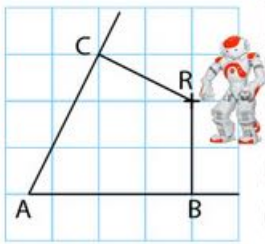
\includegraphics[width=4cm]{9_1_robot.png}
\end{center}

Le robot se trouve-t-il à même distance des droites $(AB)$ et $(AC)$ ?
\end{document}
